% !TeX program = xelatex
\documentclass[3pt,landscape]{article}
\usepackage{multicol, calc, ifthen, amsmath, amsthm, amsfonts, amssymb, color, graphicx, hyperref, fontspec, xunicode}

\usepackage[landscape]{geometry}

\defaultfontfeatures{Mapping=tex-text,Scale=MatchLowercase}
\ifthenelse{\lengthtest { \paperwidth = 11in}}
    { \geometry{top=.3in,left=.3in,right=.3in,bottom=.3in} }
    {\ifthenelse{ \lengthtest{ \paperwidth = 297mm}}
        {\geometry{top=1cm,left=1cm,right=1cm,bottom=1cm} }
        {\geometry{top=1cm,left=1cm,right=1cm,bottom=1cm} }
    }
\pagestyle{empty}
\makeatletter
\setmainfont{Source Sans Pro}
\setmonofont{Menlo}
\DeclareMathSizes{3}{3}{2}{1}
\DeclareMathOperator{\atan}{atan}

\renewcommand{\section}{\@startsection{section}{1}{0mm}{-1ex plus -.5ex minus -.2ex}{0.5ex plus .2ex}{\normalfont\large\bfseries}}
\renewcommand{\subsection}{\@startsection{subsection}{2}{0mm}{-1explus -.5ex minus -.2ex}{0.5ex plus .2ex}{\normalfont\normalsize\bfseries}}
\renewcommand{\subsubsection}{\@startsection{subsubsection}{3}{0mm}{-1ex plus -.5ex minus -.2ex}{1ex plus .2ex}{\normalfont\small\bfseries}}
\makeatother
\setcounter{secnumdepth}{0}
\setlength{\parindent}{0pt}
\setlength{\parskip}{0pt plus 0.5ex}
\hypersetup{colorlinks=true, urlcolor=blue}
\def\ci{\perp\!\!\!\perp}

%%%%%%%%%%%%%%%%%%%%%%%%%%%%%%%%%%%%%%%%%%%%%%%%%%

\begin{document}
\raggedright
\footnotesize

\begin{multicols}{3}
\setlength{\premulticols}{1pt}
\setlength{\postmulticols}{1pt}
\setlength{\multicolsep}{1pt}
\setlength{\columnsep}{2pt}

\begin{center}
    \Large{\underline{Computational Photography Field Guide}} \\
\end{center}
\begin{center}
    Written by: \href{http://krishna.im}{Krishna Parashar}\\
    Published by: \href{http://www.atrus.co}{Atrus}\\
\end{center}

%%%%%%%%%%%%%%%%%%%%%%%%%

\section*{Capturing Light}
The word \textbf{Photography} comes from \textbf{Photo} meaning light \& \textbf{Graphy} meaning drawing.

The \textbf{Iris} controls the \textbf{Pupil} which is like the aperture that projects light to the \textbf{Retina} which is like film. The retina is composed of two light sensitive receptors: 

% \begin{itemize}
% \item \textbf{Rods} that are rod-shaped, highly sensitive, usually operate at night, and only provide gray-scale vision. Range: $10^{-5}$ to $10$ lamberts. 
% \item \textbf{Cones} that are cone shaped, not very sensitive, operate in high lighting, and allow us to see color. Range: $10^{-9}$ to $10^{-5}$lamberts.
% \end{itemize}

\textbf{Rods} that are rod-shaped, highly sensitive, usually operate at night, and only provide gray-scale vision. Range: $10^{-5}$ to $10$ lamberts. \textbf{Cones} that are cone shaped, not very sensitive, operate in high lighting, and allow us to see color. Range: $10^{-9}$ to $10^{-5}$lamberts.


We primarily see visible light because that is the color spectrum the sun radiates. 

Any patch of light can be completely described by its spectrum. 
If we plot the Wavelength by the number of Photons we get some interesting properties

% \begin{itemize}
% \item The \textbf{Mean} of the distribution is the \textbf{Hue} of the patch. (BGR)
% \item The \textbf{Variance} of the distribution is the \textbf{Saturation} of the patch. (L, M, H)
% \item The \textbf{Area} of the distribution is the \textbf{Brightness} of the Images. (Dark to Bright)
% \end{itemize}

The \textbf{Mean} of the distribution is the \textbf{Hue} of the patch. (BGR) The \textbf{Variance} of the distribution is the \textbf{Saturation} of the patch. (L, M, H). The \textbf{Area} of the distribution is the \textbf{Brightness} of the Images. (Dark to Bright)

We have three types of cones (S, M, L). The M \& L cones overlap a lot to help us see bright red and green things. Since there are a lot of spectra we can't represent, distinguishing information is lost and when two such spectra is indistinguishable we call it a \textbf{Metamer}. We don't have color constancy (seeing an non varying color despite the environment of observation). Depending upon lighting we see different hues of colors. 

% \subsection*{White Balancing}
% \begin{itemize}
% \item Manually: We choose a color-neutral object in photos and normalize 
% \item Automatically 1: \textbf{Gray World} is to force average color of scene to gray. 
% \item Automatically 2: \textbf{White World} is to force brightest object to white. 
% \end{itemize}

\subsection*{White Balancing}
Manually: We choose a color-neutral object in photos and normalize. Automatically 1: \textbf{Gray World} is to force average color of scene to gray. Automatically 2: \textbf{White World} is to force brightest object to white. 

A \textbf{Bayer Filter} is a physical part of camera that is used so we can have one sensor instead of three. Generally the sensors on the CMOS array are split into 2x2 array clockwise as green, blue, green, red. More greens because we are more sensitive to green light (especially in luminance) and thus allow us to see sharper images. A \textbf{Bayer Grid} allows you to estimate the R \& B values from the G from neighboring values and generally average them to determine the values (complex camera and algorithms allow you to loose less detail, especially on edges) and convert it to a smooth continuum. This process is called \textbf{demosaicing}. RAW images allows you to do this manually. 

Color in an image is defined with the third dimension as \textbf{RGB}.

We can use \textbf{HSV} to allow is to set the Hue, Saturation, and Value (Intensity) of a pixel. 

%% LAB Color Space

To compare RBG channels and see pixel similarities we can use: 

\begin{itemize}
\item \textbf{Sum of Square Differences} is defined as $ssd(u,v) = \sum_{(x,t) \epsilon n}^{} [I(u+x, v+y)-P(x,y)]^2$
\item \textbf{Normalized Correlation} is used over SSD because it normalized the values so image is invariant over intensity.
\end{itemize}


%%%%%%%%%%%%%%%%%%%%%%%%%

\section*{The Camera}
Put Optical Center (Center of Projection) at origin. Put image plane (projection plane) in front of COP.
If you make aperture too small you get diffraction effects. Lenses help you focus. $1/f = 1/d_0 + 1/d_i$.
FOV is $\arctan{d/{2f}}$
Lenses can cause chromatic aberration or color fringes near edges of image due to glass. Sometimes radial distortion.


\section*{Transformations}

You can turn any univariate function as a sum of sines and cosines of different frequencies. $A\sin(\omega x + \phi)$

Gaussian $= G_{\sigma} = ({{1}/{2\pi \sigma^2}})e^{-{x^2 + y^2}/{2 \sigma^2}}$
\begin{verbatim}
gaussian(img):
	n, m = im.shape
	g = gauss_kernel(m, n, sigma)
	g_freq = get_freq(fft.ifftshift(g))
	c_freq = get_freq(im)
	return np.abs(fft.ifft2(fft.ifftshift(c_freq*g_freq)))
\end{verbatim}

$F[g*h] = F[g]F[h]$
$F^{-1}[gh]=F^{-1}[g]*F^{-1}[h]$
Convolution in spatial domain is equivalent to multiplication in frequency domain. It is both commutative and associative.

Convolving twice with Gaussian of width $\sigma$ is like convolving once with kernel of width $\sigma \sqrt{2}$.

To make smaller image, take Gaussian than subsample. 

\textbf{Image Filtering} is changing the range of the image $g(x)=T(f(x))$
\textbf{Image Warping} is changing the domain of the image $g(x)=f(T(x))$

\textbf{Kernel Convolution} is the process of applying a matrix (generally 3x3) to another matrix (such as an image). We basically:
\begin{enumerate}
\item Take our transformation matrix, and flip it over vertically and horizontally 
\item Slide it over each pixel in the image such that the image pixel is in the center of the transformation matrix. 
\item Multiply each value surrounding that image pixel by the corresponding value in the transformation matrix, for example the pixel to the left of the current pixel pixel in the image array would be multiplied by the pixel to the left of the current center value in the transformation matrix. 
\item We pad pixel in the image array with zero values thus ignore them, or mirror the pixel so the the transformation matrix always has something to multiply with. 
\item We then sum all the value in the transformation matrix (after it is multiplied by the original values) and divide by the number of values in the transformation matrix. 
\item We then replace that pixel in a \textbf{new image} (so we don't mess up our image) with the resulting value.
\end{enumerate}

Non-convolution is cross correlation (just dot product).

Properties of linear transformations are origin maps to origin, Lines map to lines, Parallel lines remain parallel, Ratios are preserved, Closed under composition
% \end{itemize}

Affine transformations are combinations of Linear transformations, and Translations
% \end{itemize}
Properties of affine transformations:
% \begin{itemize}, 
Origin does not necessarily map to origin, Lines map to lines, Parallel lines remain parallel, Ratios are preserved, Closed under composition, Models change of basis
% \end{itemize}

Projective transformations are combos of Affine transformations, and Projective warps.
% \end{itemize}

Properties of projective transformations:

% \begin{itemize}, 
Origin does not necessarily map to origin, Lines map to lines, Parallel lines do not necessarily remain parallel, Ratios are not preserved, Closed under composition, Models change of basis
% \end{itemize}
\subsection*{Common Filters}
% \begin{itemize}

Scaling
$\begin{bmatrix} 
x'\\ 
y'\\
\end{bmatrix} = \begin{bmatrix} 
a & 0 \\ 
0 & b \\
\end{bmatrix}\begin{bmatrix} 
x\\ 
y\\
\end{bmatrix}$

2-D Rotation
$\begin{bmatrix} 
x'\\ 
y'\\
\end{bmatrix} = \begin{bmatrix} 
cos(\theta) & -sin(\theta) \\ 
sin(\theta) & cos(\theta) \\
\end{bmatrix}\begin{bmatrix} 
x\\ 
y\\
\end{bmatrix}$

$R^{-1} = R^{T}$

Shear
$\begin{bmatrix} 
x'\\ 
y'\\
\end{bmatrix} = \begin{bmatrix} 
a & sh_x \\ 
sh_y & b \\
\end{bmatrix}\begin{bmatrix} 
x\\ 
y\\
\end{bmatrix}$

Scaling
$\begin{bmatrix} 
x'\\ 
y'\\
\end{bmatrix} = \begin{bmatrix} 
-1 & 0 \\ 
0 & 1 \\
\end{bmatrix}\begin{bmatrix} 
x\\ 
y\\
\end{bmatrix}$


Translation
$\begin{bmatrix} 
1 & 0 & t_x \\ 
0 & 1 & t_y \\
0 & 0 & 1 \\
\end{bmatrix}$

Mean Blur
$\begin{bmatrix} 
1 & 1 & 1 \\ 
1 & 1 & 1 \\
1 & 1 & 1 \\
\end{bmatrix}$

Gaussian Blur
(less weight as you move from center)
$\begin{bmatrix} 
1 & 2 & 1 \\ 
2 & 4 & 2 \\
1 & 2 & 1 \\
\end{bmatrix}$
\\
Use on black \& white images; blur before to remove high frequency noise; to find total gradient use $\atan(G_y)/(G_x)$.

Sobel Operator <$G_x$> 
$\begin{bmatrix} 
-1 & 0 & 1 \\ 
-2 & 0 & 2 \\
-1 & 0 & 1 \\
\end{bmatrix}$

Sobel Operator <$G_y$> 
$\begin{bmatrix} 
-1 & -2 & 1 \\ 
0 & 0 & 0 \\
1 & 2 & 1 \\
\end{bmatrix}$



\subsection*{Edge Detectors}


\textbf{Canny Edge Detector} For when you want finer edges on high res images, uses hysteresis thresholding on output from Sobel Edge Detector ($G_x, G_y$) with arctan to find orientation. Thresholding work by setting a value between (0, 255) and allow edge response to pass though which are over our higher threshold, reject those below lower threshold, allow value in between if they are connected to values that make it above higher threshold. 




% \section*{Image Blending}

% \section*{Warping}

% \section*{Morphing}

% \section*{Faces}
Objects don't span subspaces, colors do. 
% \subsection*{Principal Component Analysis}
% - Image Composites
% - Averaging Faces
% - Appearance vs Shape Vector


% \section*{Video Textures}

% \section*{Internet Data}

% \section*{Modeling Light}



% \section*{Image Mosaics}
% \subsection*{Homographies}
% \subsection*{RANSAC}





\section*{Projects}
\subsection*{Colorizing}
\begin{itemize}
\item  Digitized Prokudin-Gorskii glass plate images and automatically produce a color image with as few visual artifacts as possible/
\item Split Image into three channels.
\item Approach \#1: naive brute-force method that moves the red and green channels by [-15, 15] pixels in each direction, comparing them with the blue channel, and using the alignment which produced the lowest l2 norm with that blue channel's image. Inefficient for large images. 
\item Approach \#2: Dynamic programming + image pyramid scheme. Image pyramid (image at different scales at different recursive calls, scaled by a factor of 2 at each level, start processing at coarsest level (smallest image with naive SSD) so we do most of the work when it is cheapest, and look only at neighbors at the finer levels). 
\item If image dimensions were of powers of 2, and assuming that the subproblem returned the best alignment, then the alignment of the image at that current level can only be at most 1 pixel off from the displacement of the subproblem level. This is because the larger image has 4 pixels wherever the smaller had 1 pixel, so the best alignment must be in a displacement at most 1 pixel away (including diagonally) from the result of the subproblem. This means a total of 3x3=9 alignment checks per level. However, because the image dimensions are not always powers of 2, checking a distance of 2 pixels away worked better (17/18 images aligned correctly). For example, a 5x5 image divided in half would become a 2x2 image, which means the alignment can now be at most 2 pixels away from the displacement of the level below.

\end{itemize}

\subsection*{Pinhole Camera}
\begin{itemize}
\item We use this equation to find the diameter of the pinhole $d = \sqrt{2f\lambda}$ where $f$ is the focal length and $\lambda$ is 550nm. 
\item Need slow shutter speed and higher ISO. 
\item Larger aperture (like $f/2.8$) means smaller depth of field.  
\end{itemize}

\subsection*{Frequencies}
\begin{itemize}
\item \textbf{Unsharp Masking} increases contrast around edges and can make things look sharper. Convolve an image I with a gaussian to create a blurrier, low-passed version of I, called L. An approximation to the high pass version of the image I would be H = I - L. Add an arbitrary amount of the high frequencies back to the original image, has the effect of increasing contrast around the edges and in most cases makes the image look better. The final image would be F = I + alpha * H, where alpha is a parameter to tune.

\item To blend 2 images seamlessly, decompose the images into Laplacian stacks and a mask image (often binary, each pixel is a 0 or 1) into a Gaussian stack. We are more perceptive to high frequency changes, so preserve the sharp boundary between the high-frequencies by multiplying both by the non-blurred mask and combining them (by addition). The lower levels have much less information in them because they are lower frequencies, and blending the lower frequencies together with a "blurrier" mask allows for the colors and shapes to merge more effectively. For each other level we multiply the 2 images (corresponding to a level of each Laplacian stack) with an increasingly lower level of the Gaussian stack of the mask.

In other words, let 'LA' be the Laplacian stack of image A, 'LB' be the Laplacian stack of image B, 'GR' be the Gaussian stack of the mask, 'LS' be the output stack, and 'ind' be the current level of the stacks. Then each level of the output stack would be:
$LS_{ind} (i, j) = GR_{ind} (i, j) * LA_{ind} (i, j) + (1 - GR_{ind} (i, j)) * LB_{ind} (i, j)$
\item We can break an image down into frequencies by subtracting a full image from the low-passed image repeatedly to effectively band-pass the image into spatial frequencies
\end{itemize}

\subsection*{Seam Carving}
\begin{itemize}
\item Determine the 'importance' each pixel has using an \textit{energy function}. Then until image has shrunk to the desired dimension: (1) Find the lowest-importance \textit{seam} in the image. (2) Remove it.
\item Converted the image into grayscale, found the gradient of that in both the horizontal and vertical directions, find the magnitude of both of those gradient images. Then I would find either the cheapest horizontal or vertical seam. A horizontal seam is a connected path from one side of the image to the other that chooses exactly one pixel from each column. (A vertical seam is the same, but from top to bottom and with rows.) 
\item M(i,j) = minimal cost of a seam going through (i,j) (satisfying the seam properties)
\item $M(i, j)= E(i, j) + min(M(i −1, j −1),M(i −1, j),M(i −1, j +1))$
Removed the pixels from the original image by one pixel, repeating until desired size.
\item For the default energy function, I used the sobel operator to calculate $d_x$ and $d_y$ on the greyscale of the image.
\item I initially pad the image grid on both sides such that all pixels in the 2 added columns have value h, so that I can perform min operations on the borders of the pixels without having to handle the edge conditions. Why h? The maximum intensity is 1 for each pixel in the energy function image because I normalize by the highest value, so in the worst case all pixels are 1, and sum to h at the bottom of the dynamic programming algorithm.
\end{itemize}

\subsection*{Face Morphing}
Morph is a simultaneous warp of the image shape and a cross-dissolve of the image colors. Manually set correspondence which should map eyes to eyes, mouth to mouth, chin to chin, ears to ears, etc., to get the smoothest transformations. A Delaunay triangulation is found on the midpoint (average) of the corresponding points. Computing the mid-way face of the two images involves computing the average shape (a.k.a the average of each keypoint location in the two faces), the warping both faces into that shape, and averaging the colors together. The main task in warping the faces into the average shape is implementing an affine warp for each triangle in the triangulation from the original images into this new shape. This will involve computing an affine transformation matrix A between two triangles.
Affine Matrix is defined as 
$\begin{bmatrix} 
x'\\ 
y'\\
1 \\
\end{bmatrix} = \begin{bmatrix} 
a & b & c \\ 
d & e & f \\
0 & 0 & 1 \\
\end{bmatrix}\begin{bmatrix} 
x\\ 
y\\
1\\
\end{bmatrix}$
A set of these transformation matrices will then need to be used to implement an \textbf{inverse warp} (which iterates through the newly shaped image and multiply the point by the inverse matrix to find the source point, from which is "borrows" its value) for all the pixels.
Once we know how to warp the two images onto their midpoint, we can create a morph sequence by varying the weights on the average of the correspondences to get a weighted midpoint. In other words, instead of warping the images onto the exact average (i.e. both weights are 0.5) between the two images, we can morph onto any "fractional midpoint" in the range [0, 1]. They are the only parameters that will vary from frame to frame in the animation. For the starting frame, they will both equal 0, and for the ending frame, they will both equal 1. This gives rise to 2 parameters we have the option of tweaking: the warping fraction (which controls shape) and the dissolve fraction (which controls appearance, color, hue, etc.). The images are first warped into an intermediate shape configuration controlled by the warping fraction, and then cross-dissolved according to the dissolve fraction.

\subsection*{Light Fields}
\begin{itemize}
\item The objects which are far away from the camera do not vary their position significantly when the camera moves around while keeping the optical axis direction unchanged. The nearby objects, on the other hand, vary their position significantly across images. Averaging all the images in the grid without any shifting will produce an image which is sharp around the far-away objects but blurry around the nearby ones. Similarly, shifting the images 'appropriately' and then averaging allows one to focus on object at different depths.
\item To decide shift, center image as the baseline, (0, 0). The dataset includes images that are [-8, 8] on both axes. e.g. If a image 4 frames up and 2 frames to the right of the center image, translate that image by 4*scale pixels down and 2*scale pixels to the left, where scale is a parameter that varies to adjust the depth focus. 
% For example, if scale is 0, then none of the images are shifted, and averaging all of them focuses on the farther objects, since they don't change as the camera moves slightly, and the closer images appear blurry. The range of the scale parameter varies among images, since some scenes are bigger and closer to the camera than others.
\item Averaging a large number of images sampled over the grid perpendicular to the optical axis mimics a camera with a much larger aperture. This is because a larger aperture means that more light rays are being captured, from a larger area, which is similar to gathering more camera locations and averaging them. Correspondingly, using fewer images results in an image that mimics a smaller aperture. In this part of the project, I generated images which correspond to different apertures while focusing on the same point.

To change aperture average all images located at a certain distance from the center image, which is a circle with radius from 1 to 8. Here are the results of changing the aperture digitally, after the photos have been taken. The small aperture image is essentially just the center image shown above, so the full aperture (circle of images with radius = 8).
\end{itemize}

\subsection*{Image Mosaics}
\begin{itemize}
\item To warp images into alignment, recover the parameters of the transformation between each pair of images. The transformation is a homography: p’ = Hp, where H is a 3x3 matrix with 8 degrees of freedom (lower right corner is a scaling factor, so 1). To recover the homography set of (p’, p) pairs of corresponding points taken from the two images.

To find entires in H set up a linear system of n equations (i.e. a matrix equation of the form Ah = b, where h is a vector holding the 8 unknown entries of H). If n=4, the system can be solved using a standard technique. However, with only four points, the homography recovery will be very unstable and prone to noise. Therefore more than 4 correspondences should be provided producing an overdetermined system which should be solved using least-squares. Correspondences are pairs of points which should correspond in both images. 

We start with an unknown 3x3 transformation matrix. Our goal is to find the transformation matrix such that for some number of correspondences, the error between p' and Hp (from the equation p' = Hp above) is minimized; that is, transforming each of the correspondences in the first image should get as close as possible to what we want them to correspond to in the 2nd image. By filling in the values (a through i) of the matrix, we can use the matrix to determine where an arbitrary pixel (x,y) would map to (x', y') as a result of this warp.
\end{itemize}
\begin{center}
    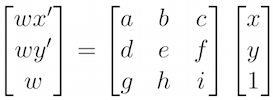
\includegraphics[height=1cm]{images/homography.png}
\end{center}
\begin{itemize}
\item This equation is for a single correspondence only. We want to solve for the values a through h in the matrix, since we can set i to be 1 because it is a scale factor. So, we can rearrange these terms to create a new matrix system b=Ah to solve for those 8 values. This gives us 2 equations for each correspondence (shown below), and more points can be added to get a better estimate of the transformation matrix (at least 4 pairs necessary, since 8 equations are needed to solve for 8 unknowns). Solving this with least squares gives us the best approximation which minimizes the error for the set of correspondences.
\end{itemize}
\begin{center}
    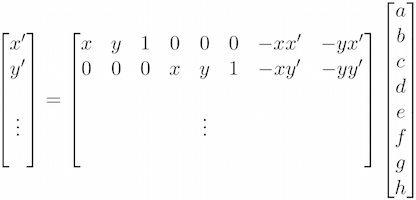
\includegraphics[height=1.5cm]{images/homography-values.png}
\end{center}
\begin{itemize}
\item Predict the size of the bounding box by piping the four corners of the image through H. Inverse warping and interpolation to compute what pixel in the first image transforms to each pixel in the second image. The interpolation avoids aliasing when resampling the image. To mark pixels which don't have any values, use alpha mask.
\item Now I can warp images so they're registered and create an image mosaic. Instead of having one picture overwrite the other, which would lead to strong edge artifacts, I first tried weighted averaging. I left one image unwarped and warped the other image(s) into its projection.

Now we need to blend them together to produce a single image. I used an alpha channel, and at every pixel where the two images overlapped, I weighted the two images equally (0.5), and kept the unique portions the same (weights of 0 or 1, opposite for each image)
\item To detect key points in each image use Harris Interest Point Detector. The idea behind this is that edges or flat surfaces are able to be shifted along at least one direction and still look the same, and may have multiple possibilities for correspondences in the other image. I used Adaptive Non-Maximal Supression to keep key points which were as spread apart from each other as possible. To compare the key points in one image to the other to select correspondences, we need to extract some sort of feature descriptor that represents each point. Then we will be able to determine the similarity between the points in each image by comparing these feature descriptors. I took the 40x40 window of pixels around each point, and downsampled by a factor of 5 so that the window was now a 8x8 block. Then I adjusted each feature descriptor to have zero mean and a variance of 1, to account for minor lighting differences.


\end{itemize}


%\rule{0.3\linewidth}{0.1pt}
\scriptsize

\end{multicols}
\end{document}
